%------------------------------------------------
\section{Динамическая апертура}
%------------------------------------------------

%------------------------------------------------
\begin{frame}[t]{Динамическая апертура}
	\vspace{-0.2cm}
	\centering
	\begin{columns}[t, onlytextwidth]
		% КОЛОНКА 1
		\begin{column}{0.33\textwidth}
			\centering
			\textbf{\scriptsize Регулярная} \\[0.1cm]
			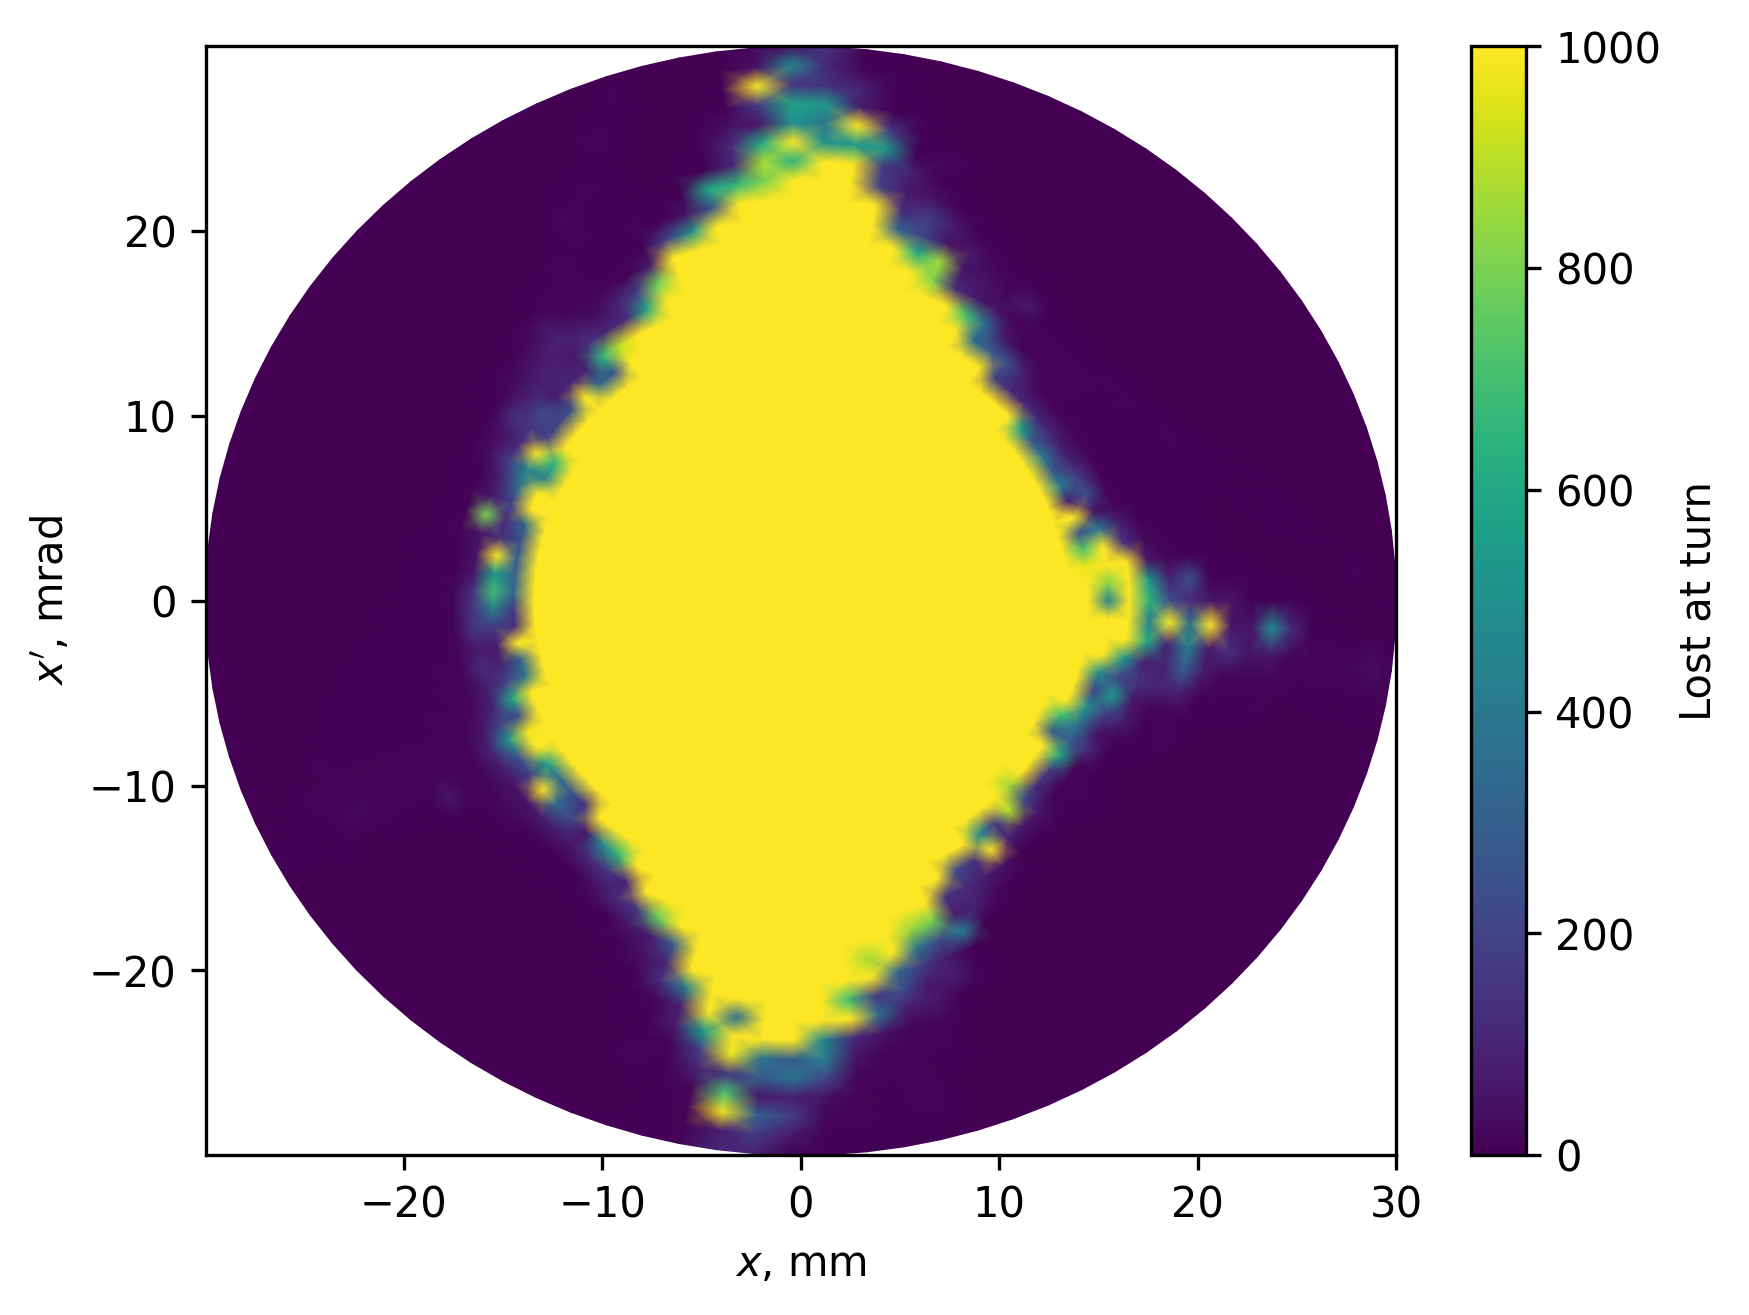
\includegraphics[height=0.37\textheight, keepaspectratio]{images/Dyn_aper_Regular_xpx_0_0} \\
			\vspace{0.1cm}
			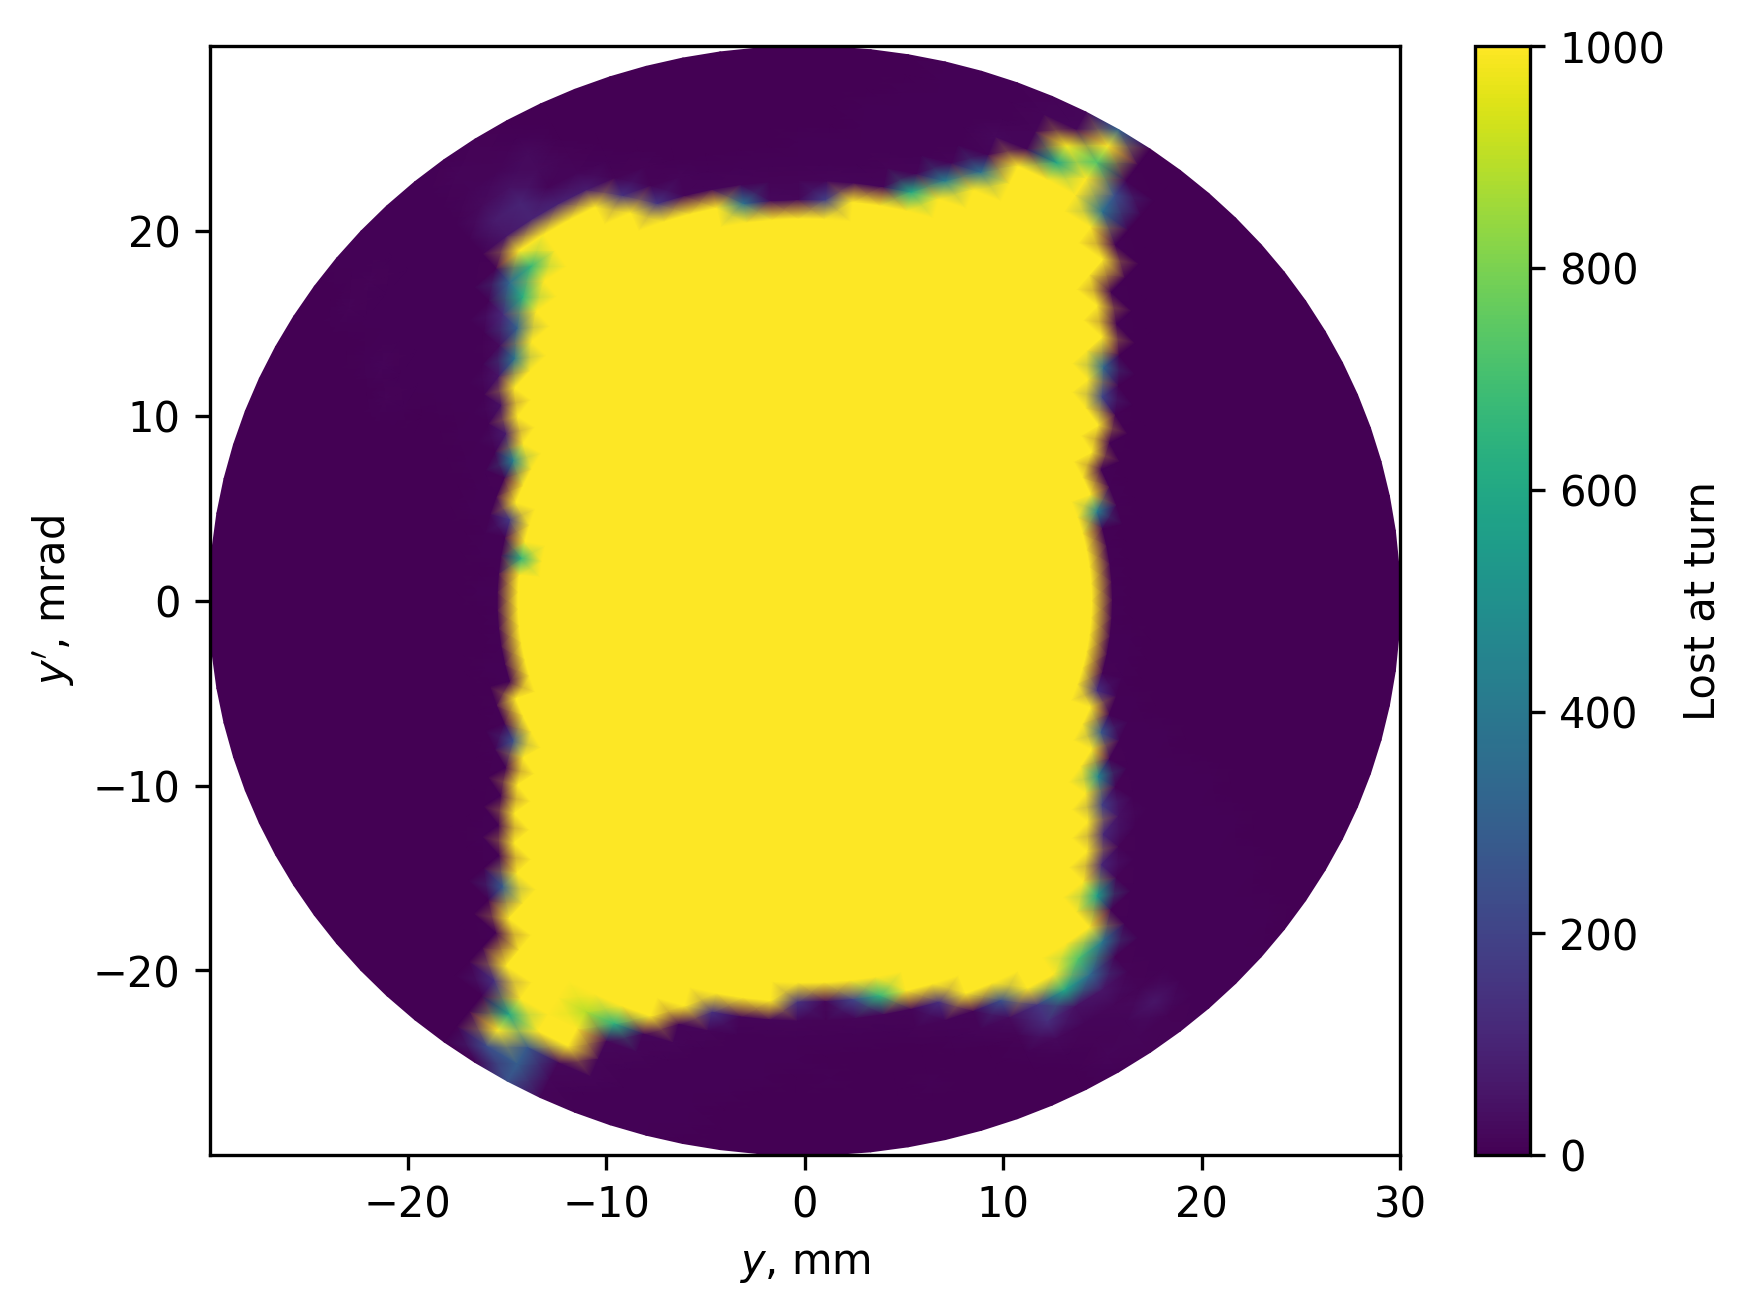
\includegraphics[height=0.37\textheight, keepaspectratio]{images/Dyn_aper_Regular_ypy_0_0}
		\end{column}
		% КОЛОНКА 2
		\begin{column}{0.33\textwidth}
			\centering
			\textbf{\scriptsize Резонансная} \\[0.1cm]
			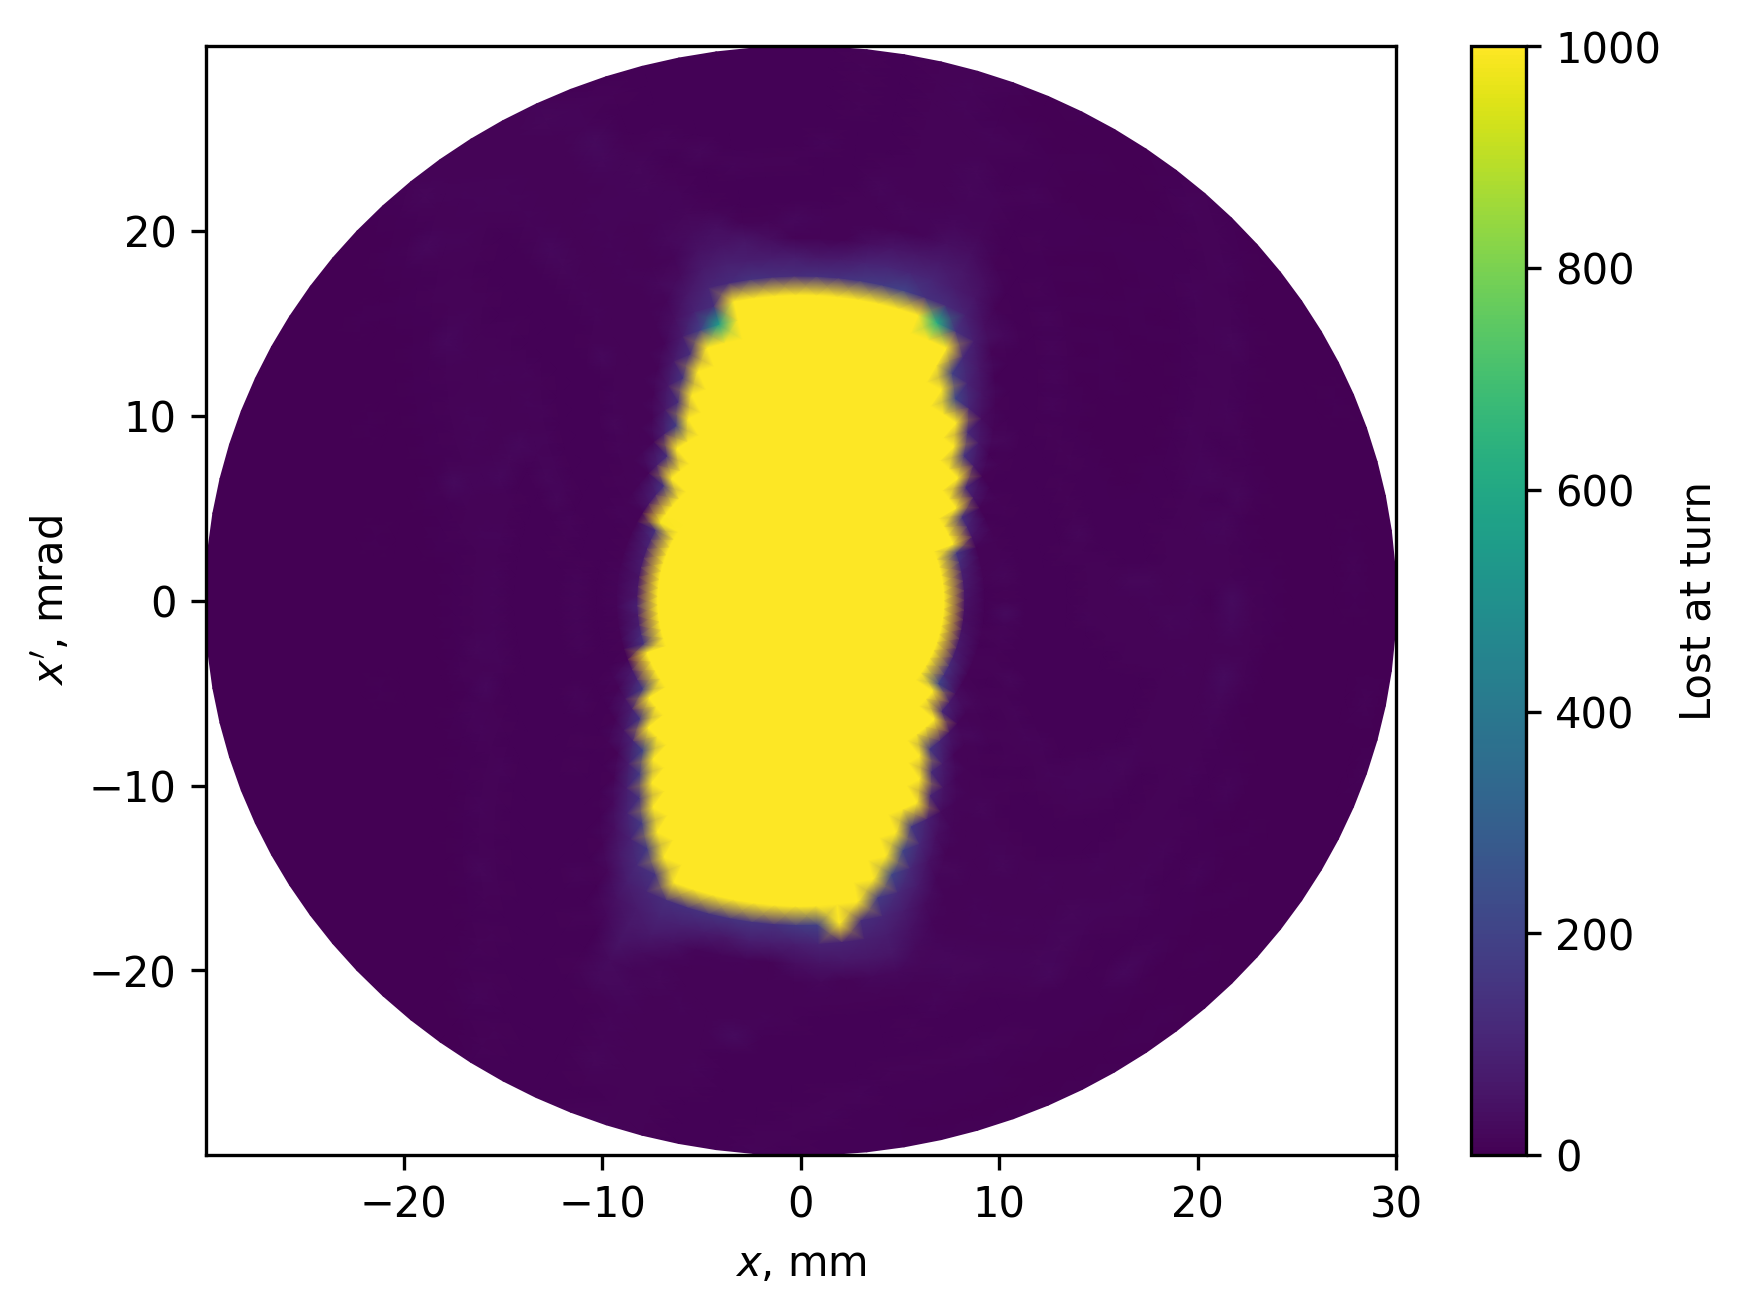
\includegraphics[height=0.37\textheight, keepaspectratio]{images/Dyn_aper_Resonant_xpx_0_0} \\
			\vspace{0.1cm}
			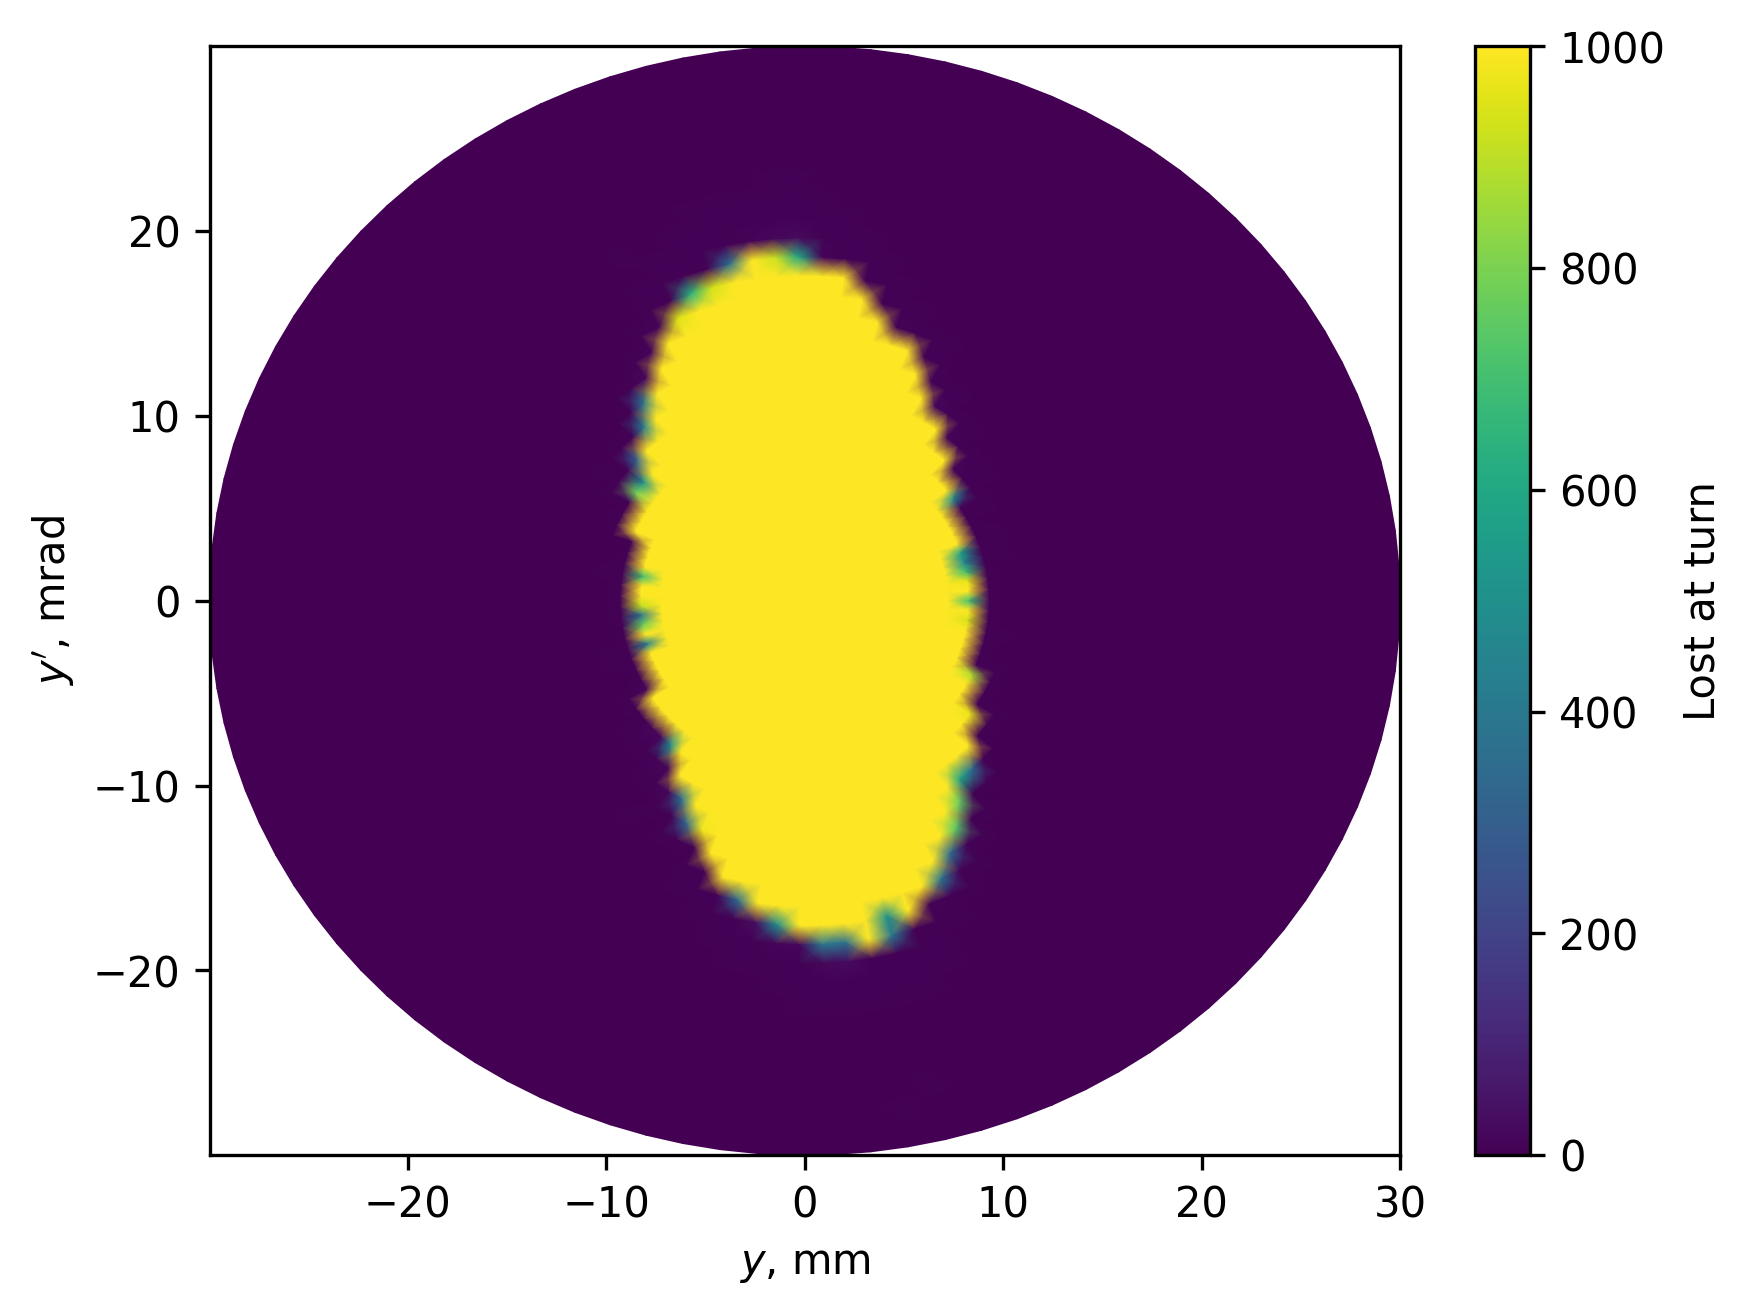
\includegraphics[height=0.36\textheight, keepaspectratio]{images/Dyn_aper_Resonant_ypy_0_0}
		\end{column}
		
		% КОЛОНКА 3
		\begin{column}{0.33\textwidth}
			\centering
			\textbf{\scriptsize Комбинированная} \\[0.1cm]
			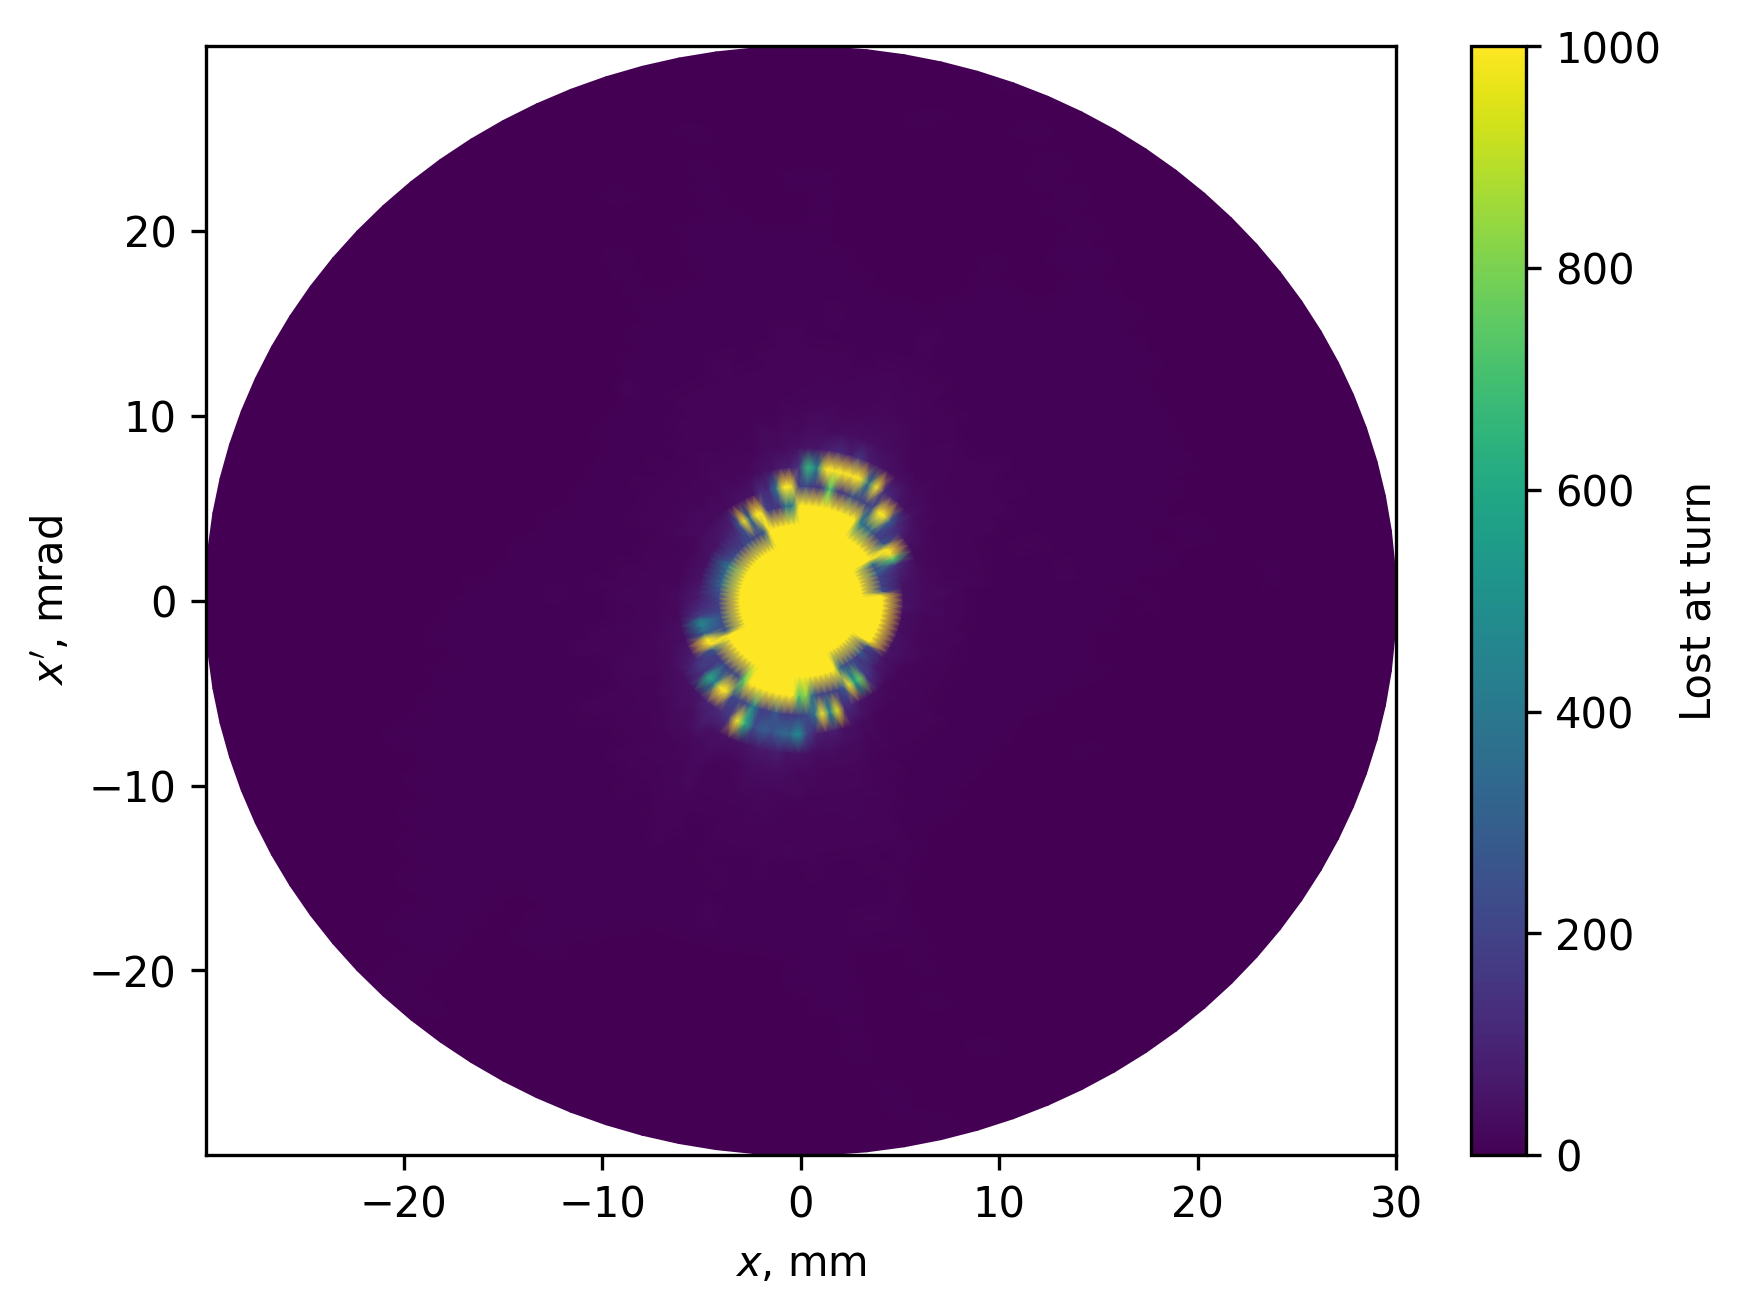
\includegraphics[height=0.37\textheight, keepaspectratio]{images/Dyn_aper_Combined_xpx_0_0} \\
			\vspace{0.1cm}
			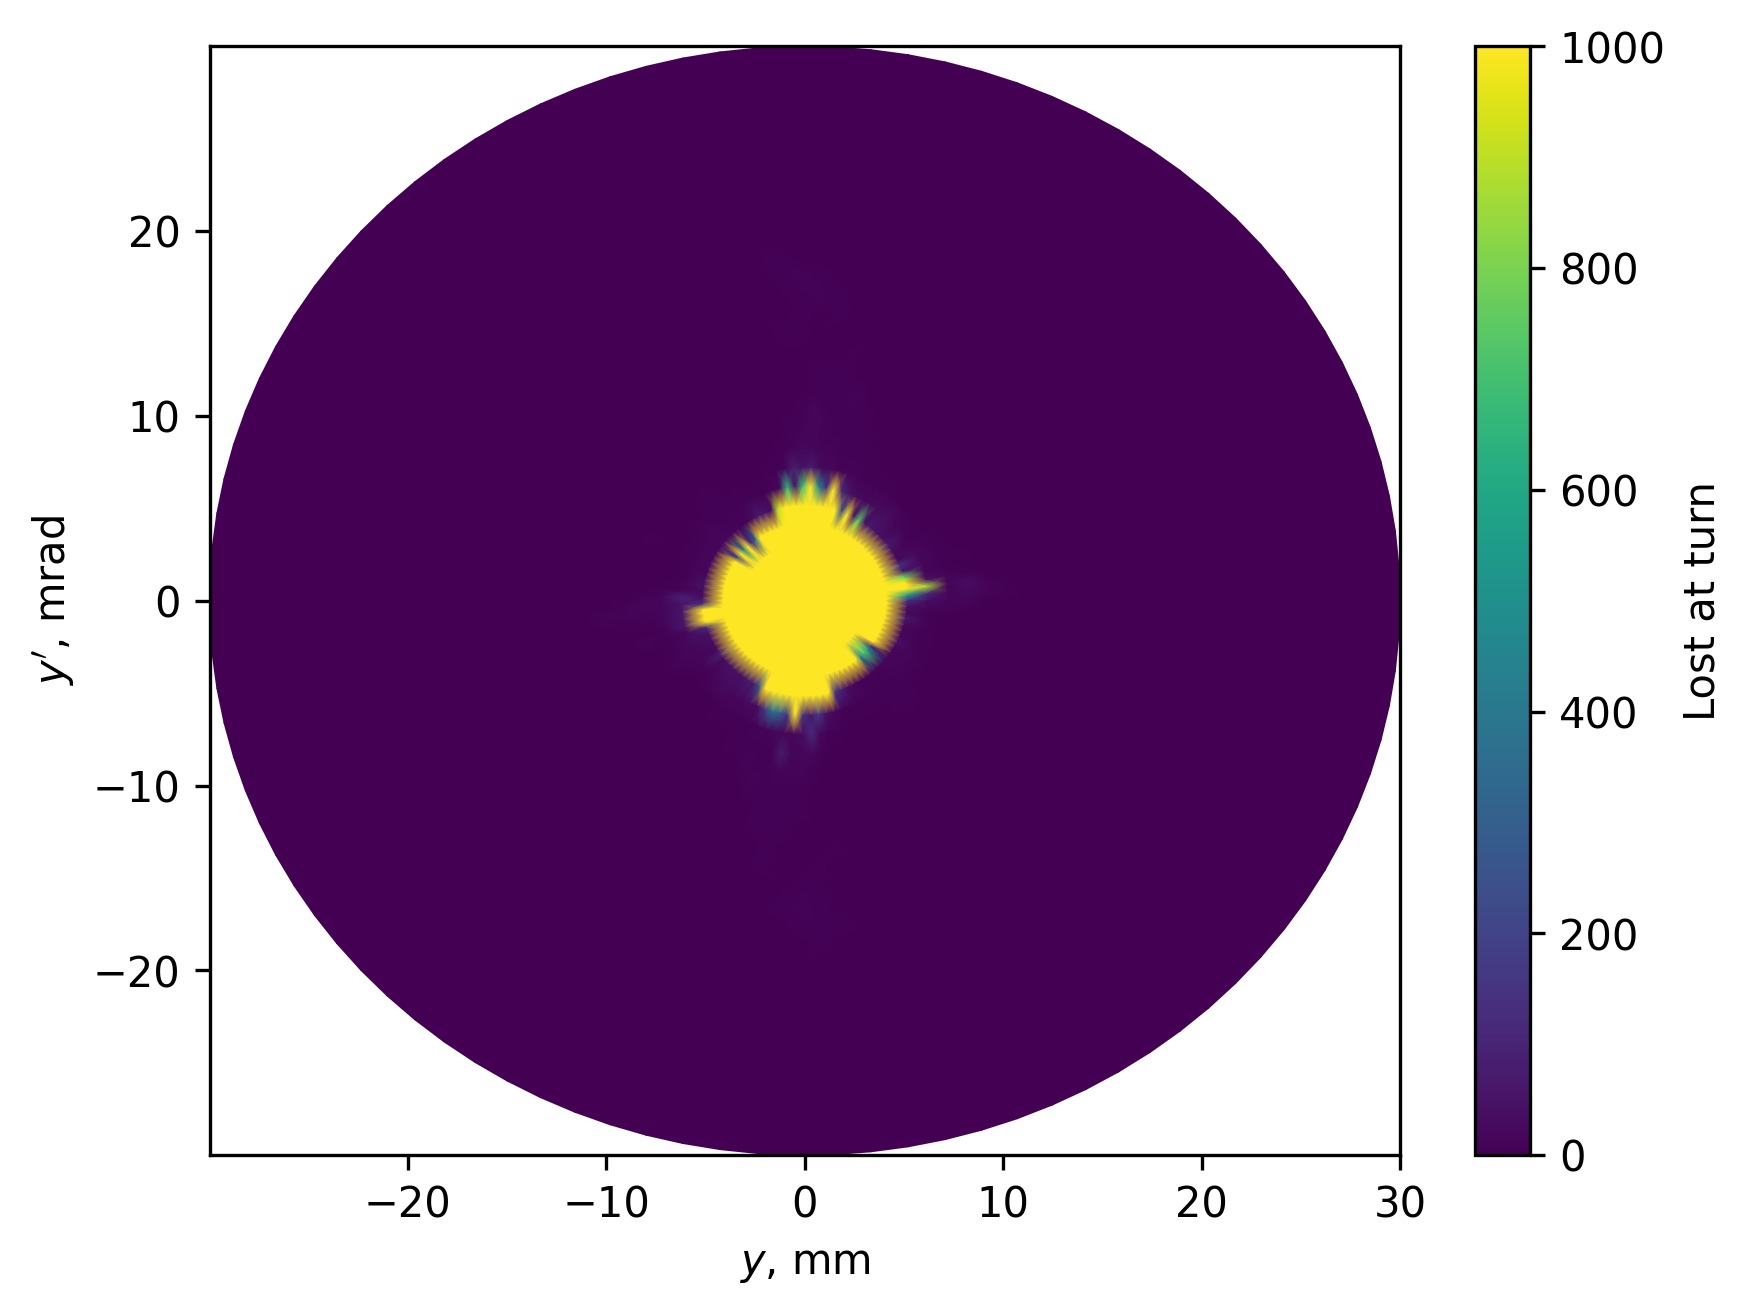
\includegraphics[height=0.37\textheight, keepaspectratio]{images/Dyn_aper_Combined_ypy_0_0}
		\end{column}
	\end{columns}
\end{frame}

%------------------------------------------------
\section{Диаграмма частот}
%------------------------------------------------

\begin{frame}[t]{Область разброса бетатронных частот при скачке критической энергии}
	\par Скачок критической энергии в \textbf{регулярной} структуре NICA осуществляется сдвигом градиента в фокусирующих квадруполях.
	\begin{equation}
		\gamma_{\text{tr}} \sim Q_{x}
	\end{equation}

	\vspace{0.1cm} % Небольшой отступ для красоты
	
	\begin{columns}[c]
		\begin{column}{0.3\textwidth}
			\centering
			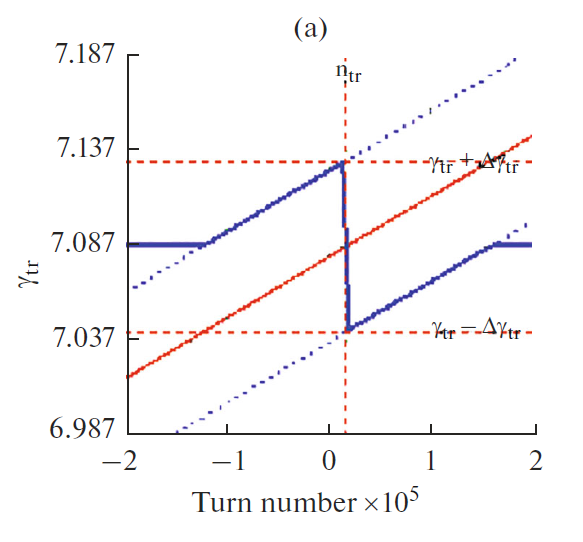
\includegraphics[width=\linewidth]{images/jump}
		\end{column}
		
		\begin{column}{0.65\textwidth}
			\centering
			% Добавляем ограничение по высоте (height), сохраняя пропорции
			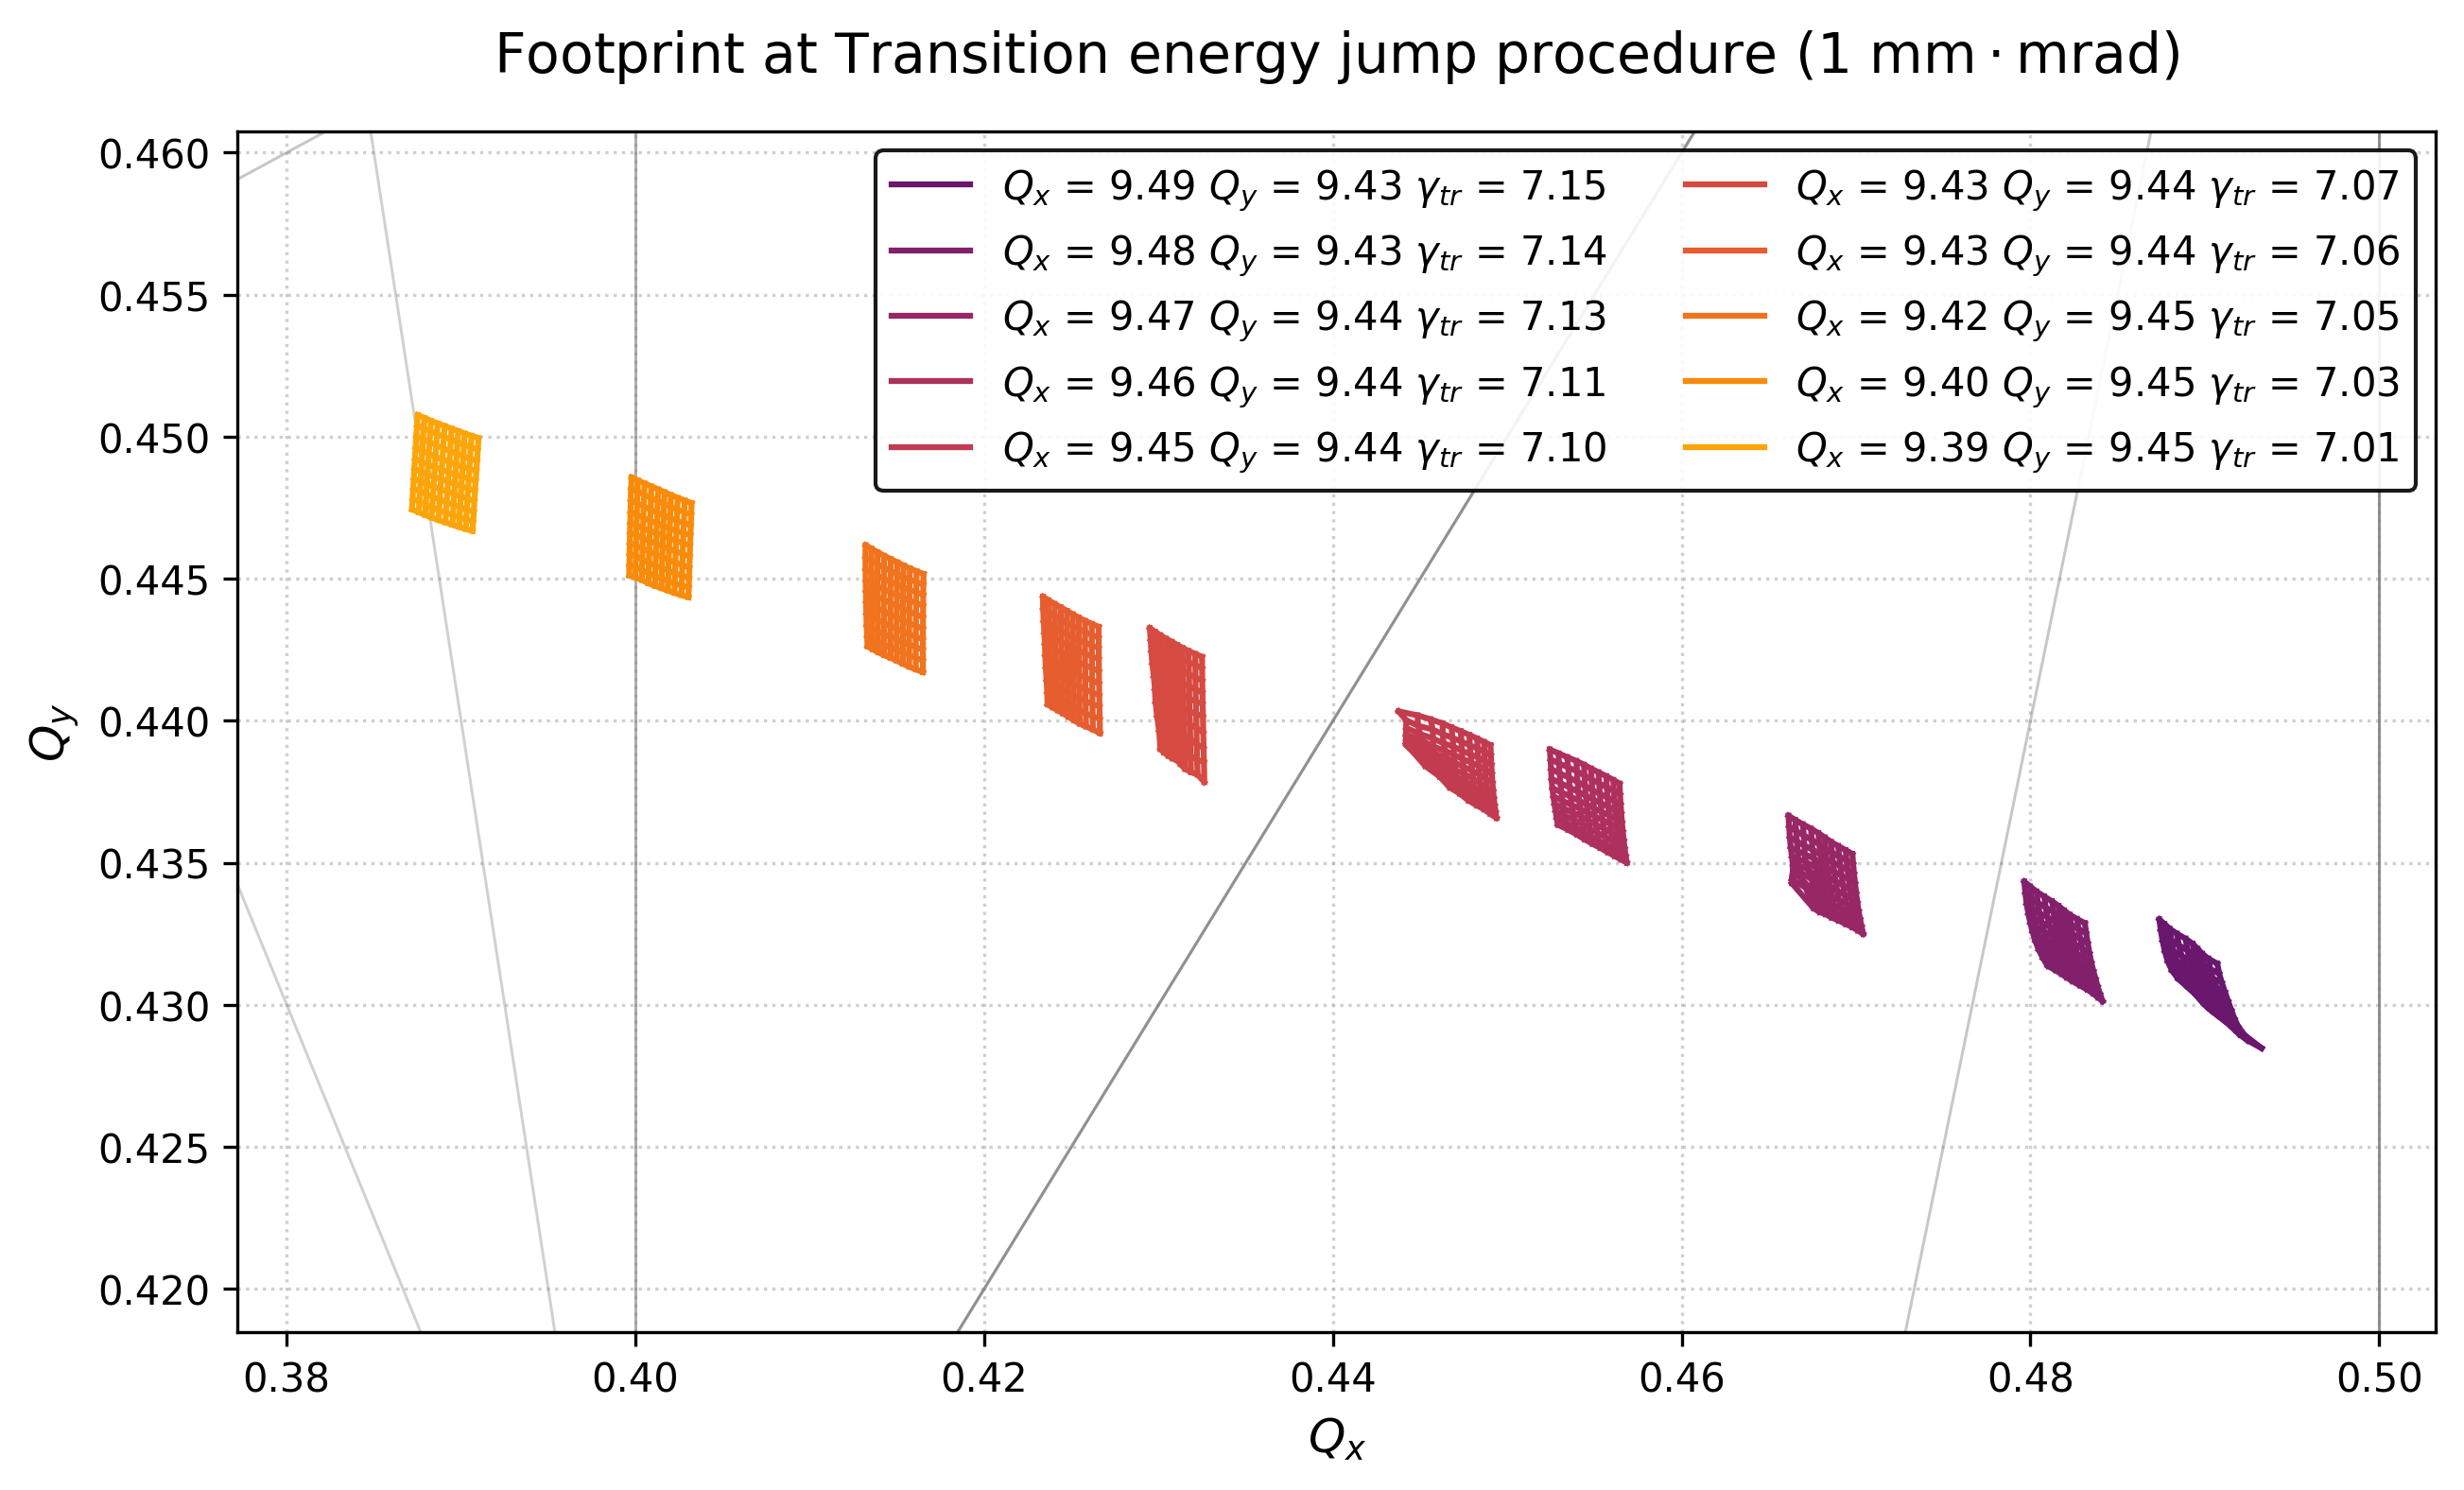
\includegraphics[width=\linewidth, height=0.6\textheight, keepaspectratio]{images/footprint_jump}
		\end{column}
	\end{columns}
\end{frame}

